
\section{Implementation}
\label{s:imp}

This section describes the {\it Runtime}, {\it Encoder}, and  {\it Query
Executor}  components in greater detail.



\subsection{Runtime}

In SciDB (and our prototype), we automatically store black-box lineage by using
write-ahead logging, which guarantees that black-box lineage is written before
the array data, and is ``no overwrite'' on updates.  Region lineage is stored
in a collection of BerkeleyDB hashtable instances.  We use BerkeleyDB to store
region lineage to avoid the client-server communication overhead of interacting
with traditional DBMSes.  We turn off fsync, logging and concurrency control to
avoid recovery and locking overhead.  This is safe because the region lineage
is treated as a cache, and can always be recovered by re-running operators.  

The runtime allocates a new BerkeleyDB database for each operator instance that
stores region lineage.  Blocks of region pairs are buffered in memory, and
bulk encoded using the {\it Encoder}.  The data in each region pair is stored
as a unit (\sys{} does not optimize across region pairs), and the output and
input cells use separate encoding schemes.  The layout can be optimized for
backward or forward queries by respectively storing the output or input cells
as the hash key.  On a key collision, the runtime decodes, merges, and
re-encodes the two hash values.  The next subsection describes how the {\it
Encoder} serializes the region pairs. 


\subsection{Encoder}
\label{s:encoder}



While Section~\ref{s:storagemodel} presented efficient ways to represent region
lineage, \sys{} still needs to store cell coordinates, which can easily be
larger than the original data arrays.  The {\it Encoder} stores the input and
output cells of a region pair (generated by calls to $lwrite()$) into one or
more hash table entries, specified by an {\it encoding strategy}. We say the encoding
strategy is {\it backward optimized} if the output cells  are stored in the hash key,
and {\it forward optimized} if the hash key contains input cells.  

We found that four basic strategies work well for the operators we encountered.
-- $FullOne$ and $FullMany$ are the two strategies to encode full lineage, and
$PayOne$ and $PayMany$ encode payload lineage\footnote{We tried a large number
    of possible strategies and found that complex encodings (e.g., compute and
    store the bounding box of a set of cells, $C$, along with cells in the
bounding box but not in $C$) incur high encoding costs without noticeably
reduced storage costs.  Many are also readily implemented as payload or
composite lineage}.

\begin{figure}[h!]
\begin{center}
   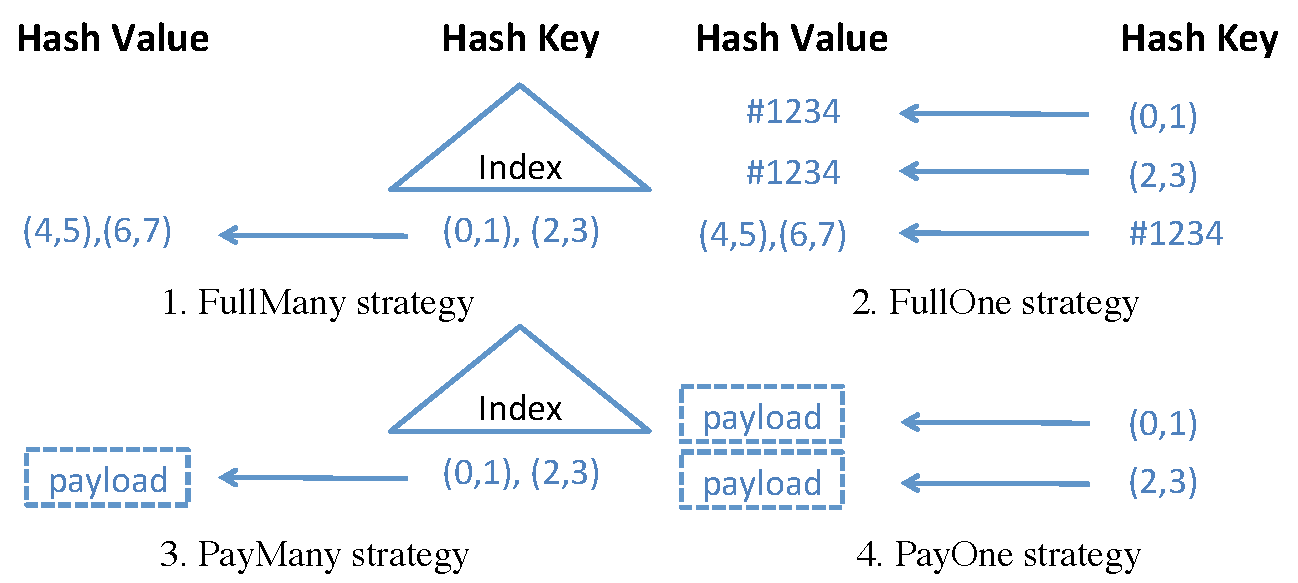
\includegraphics[width=3.1in,natwidth=8.66in,natheight=3.89in]{figures/pointer.pdf}
\caption{ Four examples of encoding strategies }
\label{f:pointer}
\end{center}
\end{figure}

Figure~\ref{f:pointer} depicts how the backward-optimied implementation of
these strategies encode two output cells with coordinates $(0,1)$ and $(2,3)$
that depend on input cells with coordinates $(4,5)$ and $(6,7)$. $FullMany$
uses a single  hash entry with the set of serialized output cells as the key
and the set of input cells as the value (Figure \ref{f:pointer}.1).  Each
coordinate is  bitpacked into a single integer if the array is small enough. We
also create an R\* Tree on the cells in the hash key to quickly find the
entries that intersect with the query. This index uses the dimensions of the
array as its keys and identifies the hash table entries that contain cells in
particular regions.  The figure shows the unserialized versions of the cells
for simplicity.  $FullMany$ is most appropriate when the lineage has high
fanout because it only needs to store the output cells once.

If the fanout is low, $FullOne$ more efficiently serializes and stores each
output cell as the hash key of a separate hash entry.  The hash value stores a reference
to a single entry containing the input cells (Figure \ref{f:pointer}.2).  This implementation doesn't need to
compute and store bounding box information 
and doesn't need the spatial index because each input cell is
stored separately, so queries execute using direct hash lookups.

For payload lineage, $PayMany$ stores the lineage in a similar manner as
$FullMany$, but stores the payload as the hash value
(Figure~\ref{f:pointer}.3).  $PayOne$ creates a hash entry for every output
cell and stores a duplicate of the payload in each hash value
(Figure~\ref{f:pointer}.4).

%In general, $ONE$ is used to
%encode small sets of cells, $MANY$ is used to encode large unique sets of
%cells, while $REF$ is used when a set of cells will be duplicated many times.


%the output cells as a single hash key and creates a spatial index on
%them (Figure \ref{f:pointer}.3), or separately by duplicating the payload for
%each output cell (Figure \ref{f:pointer}.4).  
%Figure \ref{f:pointer} depicts how four of the prevailing backward optimized
%encoding strategies encode a region pair with output cell coordinates $\{(0,1),
%(2,3)\}$ and input coordinates $\{ (4,5),$ $ (6,7) \}$.  
%\noindent {\bf ONE}: Serializes and stores each cell individually
%  by concatenating the  coordinates in each dimension.
%  If the array is small enough, we bitpack the coordinates into a
%  single integer.   \\
%\noindent {\bf MANY}: Serializes and stores the set of cells together.\\
%\noindent {\bf REF}: Stores a reference to the set of cells, which 
%  are encoded using $MANY$ and stored in a separate hash entry.\\
%\noindent {\bf BINARY}: Stores payload as a binary blob.  Reserved for payload lineage.



%We will describe the storage layouts in terms of being optimized for backward lineage
%queries.  We rewrite forward lineage queries, $lwrite(O,
%I_1,\ldots,I_n)$, into $n$ separate calls, $lwrite(I_1, O)$,\ldots,
%$lwrite(I_n, O)$.  We do this because forward queries   \srm{How are those separate calls encoded?   Why do we do
%this? I find this paragraph confusing.}







%$enc_{out}$ can take values of $ONE$, which
%creates a hash entry for each output cell and replicates the serialized input
%cells as the value of each entry, or $MANY$, which stores the output and input
%cells in a single entry, and creates a spatial index on the minimum bounding
%boxes of the output cells.  $enc_{in}$ can take the values of $MANY$, $REF$, or
%$BINARY$. $REF$ stores the cells in a separate hash entry, and keeps a
%reference to the entry with the output cells.  $BINARY$ is dedicated to payload
%data and is stored without modification.




The {\it Optimizer} picks a lineage strategy that spans the entire workflow. It
picks one or more {\it storage strategies} for each operator.  Each storage
strategy is fully specified by a  lineage mode (Full, Map, Payload,
Composite, or Black-box), encoding strategy, and
whether it is forward or backward optimized ($\rightarrow$ or $\leftarrow$).
\sys{} can use multiple storage strategies to optimize for different query types. 


\subsection{Query Execution}
\label{s:qexec}


The {\it Query Executor} iteratively executes each step in the lineage query
path by joining the lineage with the coordinates of the query cells, or the
intermediate cells  generated from the previous step.  The output at each step
is a set of cell coordinates that is compactly stored in an in-memory boolean
array with the same dimensions as the input (backward query) or output (forward
query) array.  A bit is set if the intermediate result contains the
corresponding cell.  For example, suppose we have an operator $P$ that takes as
input a $1\times 4$ array.  Consider a backwards query asking for the lineage
of some output cell $C$ of $P$.  If the result of the query is $1001$, this
means that $C$ depends on the first and fourth cell in $P$'s input.

We chose the in-memory array because many operators have large fanin or fanout,
and can easily generate several times more results (due to duplicates) than are
unique.  De-duplication avoids wasting storage and saves work.  Similarly, the
executor can close an operator early if it detects that all of the possible
cells have been generated.

We also implement an {\it entire array optimization} to speed up queries where
all of the bits in the boolean array are set.  For example, this can happen if
a backward query traverses several high-fanin operators or an all-to-all
operator such as matrix inversion.  In these cases,  calculating the lineage of
every query cell is very expensive and often unnecessary.  Many operators
(e.g., matrix multiply or inverse) can safely assume that the forward
(backward) lineage of an entire input (output) array is the entire output
(input) array.  This optimization is valuable when it can be applied -- it
improved the query performance of a forward query in the astronomy benchmark
that traverses an all-to-all-operator by 83$\times$.

In general, it is difficult to automatically identify when the optimization's
assumptions hold.  Consider a concatenate operator that takes two 2D arrays A,
B with shapes (1, n) and (1, m), and produces an (1, n+m) output by
concatenating B to A.  The optimization would produce different results, because
A's forward lineage is only a subset of the output.  We currently rely on the
programmer to manually annotate operators where the 
optimization can be applied. 

